
\begin{figure*}[t]
  \centering
  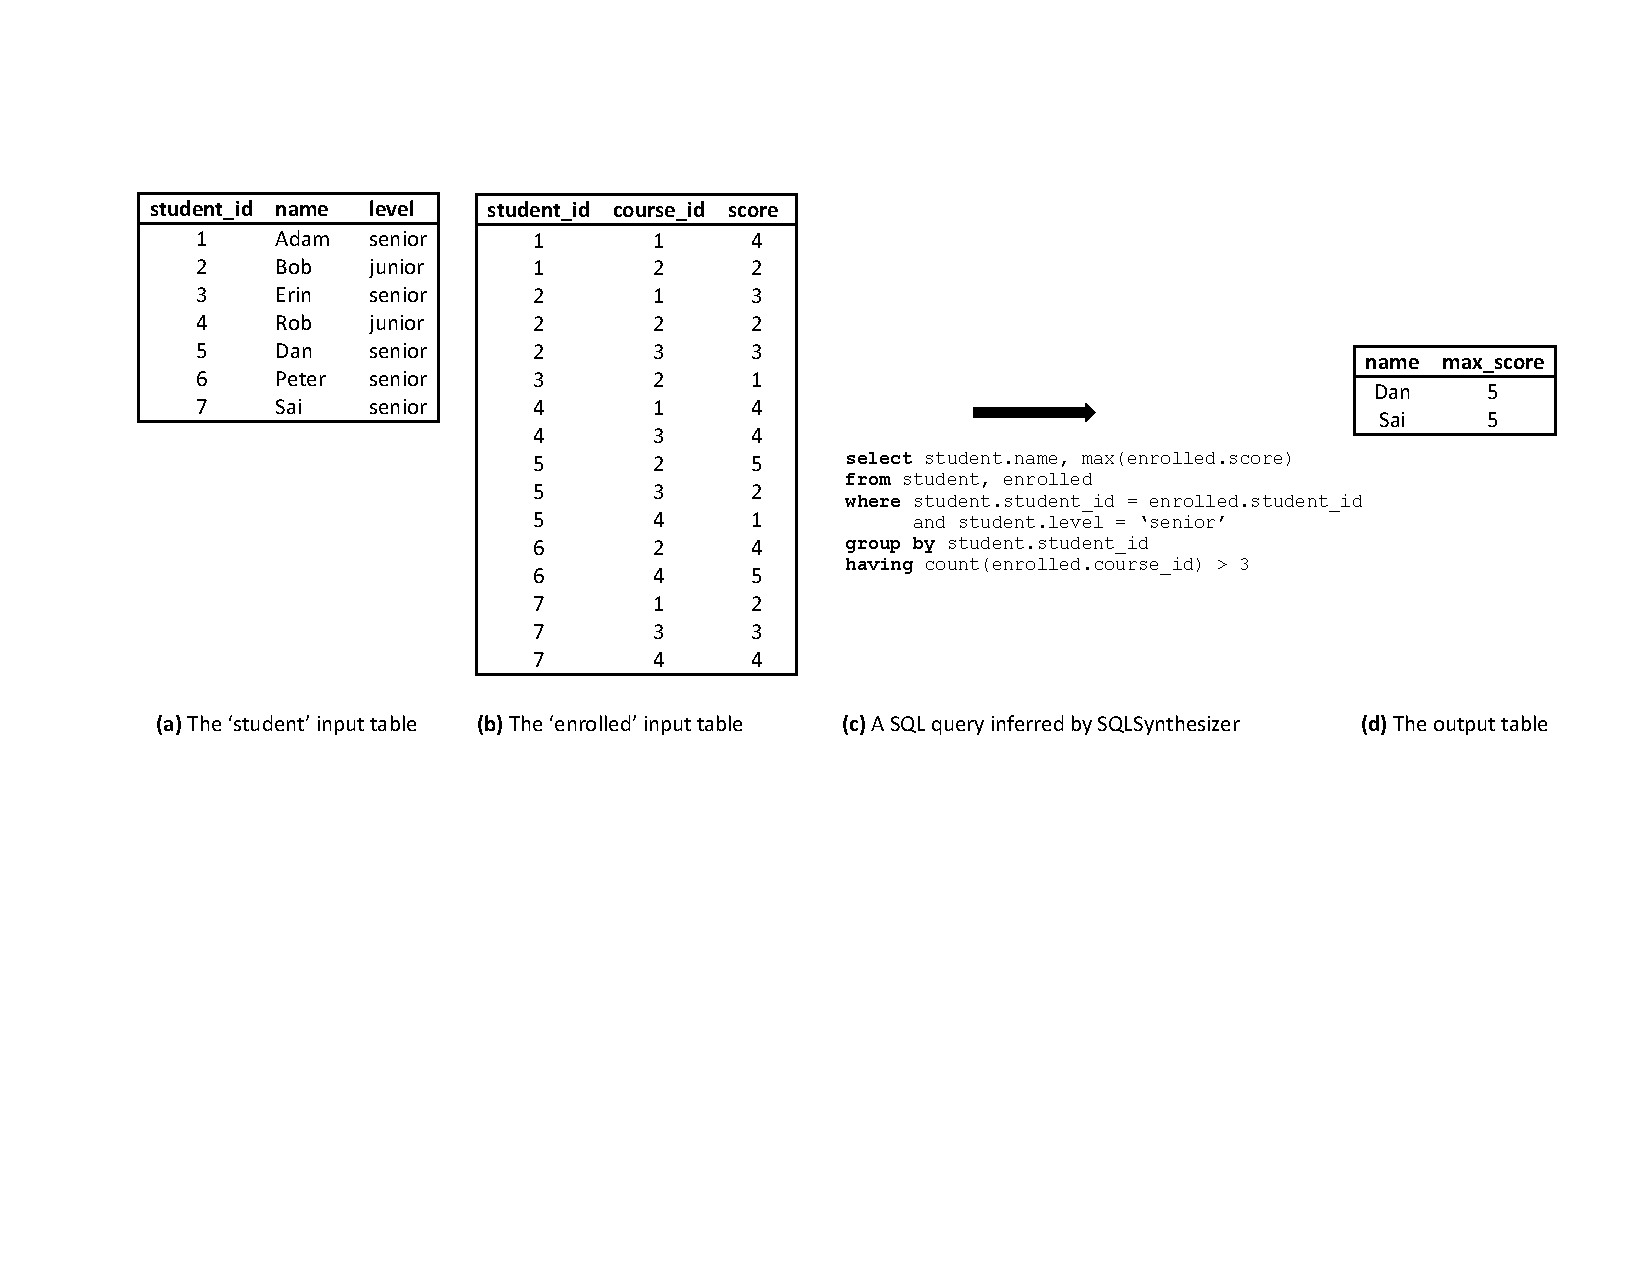
\includegraphics[scale=0.73]{motivating}
  \vspace*{-2.0ex}\caption {{\label{fig:motivating}
  Illustration of how to use \ourtool to solve the problem in Section~\ref{sec:example}.
  The user provides \ourtool with
  two input tables (shown in (a)) and an output table (shown in (c)).
  \ourtool automatically synthesizes a SQL query (shown in (b)) that
  transforms the two input tables into the output table.
}}
\vspace{-1mm}
\end{figure*}

\section{Illustrating Example}
\label{sec:example}

\vspace{-1mm}

We use an example, described below, to illustrate the use
of \ourtool. The example is taken from a classic
database textbook~\cite{cowbook} (Chapter 5, Exercise 1)
and has been simplified for illustration purpose\footnote{
This exercise defines 2 tables, whose
schemas are shown in Figure~\ref{fig:motivating}(a).}.

\begin{quote}
\textit{Find the name and the maximum course score of each senior student
enrolled in more than 2 courses.}
\end{quote}

Despite the simplicity of the problem description,
writing a correct SQL query  can be non-trivial for a typical
end-user. An end-user must carefully choose the
right SQL features and use them correctly
to fulfill the described task.
%Although most users can clearly understand the
%question, they must choose the right SQL
%features and use them correctly.

As an alternative, users can use \ourtool to obtain
the desired query.
%As illustrated in Figure~\ref{fig:motivating},
To use \ourtool, an end-user only needs to provide it with
some small, representative example input and output tables
(Figures~\ref{fig:motivating}(a) and~\ref{fig:motivating}(c)).
Then, \ourtool works in a fully-automatic, push-button
way to infer a SQL query that satisfies the given
example input and output.

 %illustrate in Figure~\ref{fig:motivating}, an alternative
%approach to write this query is to provide \ourtool
%with some representative input-output examples; and
%let \ourtool automatically automatically infer the query.

The SQL query, shown in Figure~\ref{fig:motivating}(b),
first joins two tables on the common \CodeIn{student\_id} column,
and then groups the joined results by the \CodeIn{student\_id}
column. Further, the query selects all senior
students (using a query condition in the \CodeIn{WHERE}
clause) who are enrolled in more than 2 courses
(using a condition in the \CodeIn{HAVING} clause).
Finally, the query projects the result on the
\CodeIn{student.name} column and uses the \CodeIn{MAX} aggregate
to compute the maximum course score. To the best of
our knowledge, none of the existing techniques~\cite{Tran:2009, DasSarma:2010, Harris:2011,
 Kandel:2011}
can infer this query from the given examples.

%the \CodeIn{student} with \CodeIn{enrolled} tables,
%then group bys the joined table by the \CodeIn{student\_id}
%column, and selects students enrolled in more
%than 2 courses (using the \CodeIn{having} statement).
%After that, the query further selects students
%whose level is \CodeIn{senior} and uses the \CodeIn{max}
%aggregator function to compute the maximum course score.
%\todo{the above needs polish}






